\documentclass[a4paper,12pt]{article}   % 文檔類型為article
\usepackage{setspace}
\usepackage{fontspec}% 使用系统字体
\usepackage{xeCJK}    % 提供中文支持

% 设置中文正文字体为標楷體,你需要确保系统上有標楷體字体文件
\setCJKmainfont{標楷體}

%\onehalfspacing % 1.5 倍行距,與 Word 中的默認行距相同
%\pagestyle{empty}

\setmainfont{Times New Roman}
\fontsize{12pt}{\baselineskip}   % 設置字體大小為12pt,行距為單行


\usepackage{pdfpages}
\usepackage{enumitem}
\usepackage{fontspec}
\usepackage{authblk} 
\usepackage{titlesec}
\usepackage{amssymb}
\usepackage{graphicx}
\usepackage{titlesec}
\titlespacing{\section}{0pt}{*2}{*1}
\titlespacing{\subsection}{0pt}{*2}{*1}
\titlespacing{\subsubsection}{0pt}{*2}{*1}

\usepackage{tabularx}
\usepackage{multirow}
%\usepackage{colortbl}
\usepackage{amsthm}
\usepackage{booktabs} % 用於漂亮的表格樣式


\usepackage{colortbl} % 用於表格顏色
\usepackage{xcolor}   % 用於文本顏色
\definecolor{lightgray}{gray}{0.9} % 自定義顏色

\pagestyle{plain}


\begin{document}
%\maketitle

\begin{center}
	{\fontsize{16pt}{12pt}\selectfont YOLO Object Detection on PASCAL VOC}
	
\end{center}

\hfill  B092040016 陳昱逢
	
	
\begin{center}
	Assignment 5
\end{center}

\section{實作細節}
	本次作業主要實作 You Only Look Once (YOLO) 的 loss function, Figure\ \ref{fig:loss} 呈現 YOLO 的損失函數,主要分三個部分:(1)regression loss (2)confidence loss (3) classification loss
	
	
	
\begin{figure}[htb]
  \vspace{0.1\baselineskip}  
  \centering  
  %\begin{center}
    \resizebox{0.7\textwidth}{!}{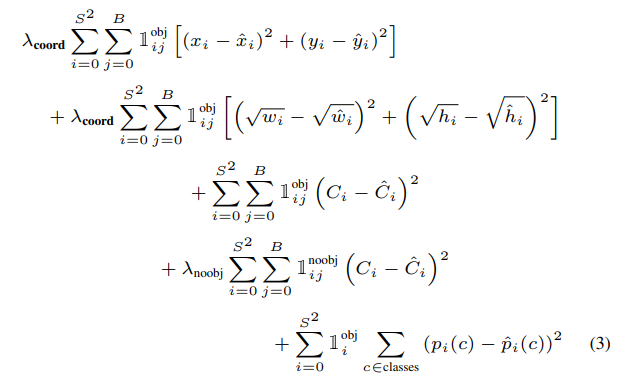
\includegraphics{loss.png}}
    \caption{YOLO loss function}
    \label{fig:loss}
  %\end{center}
  \vspace{0.1\baselineskip}
\end{figure}


在了解到 YOLO loss function 是如何運作之後,我從 YOLO loss class 的 forward function 開始實作,再依序完成呼叫到的 function,分類錯誤以及沒有物體的信心度分數都只需簡單的計算 mse loss,而regression loss以及有物體的信心分數 loss 都需經過找到每個含物體的 grid 裡面 iou 最大的 box 再分別去算對應的 loss 。 Figure\ \ref{fig:code} 呈現我的主要 YOLO loss forward funtion。

\begin{figure}[htb]
  \vspace{0.1\baselineskip}  
  \centering  
  %\begin{center}
    \resizebox{1\textwidth}{!}{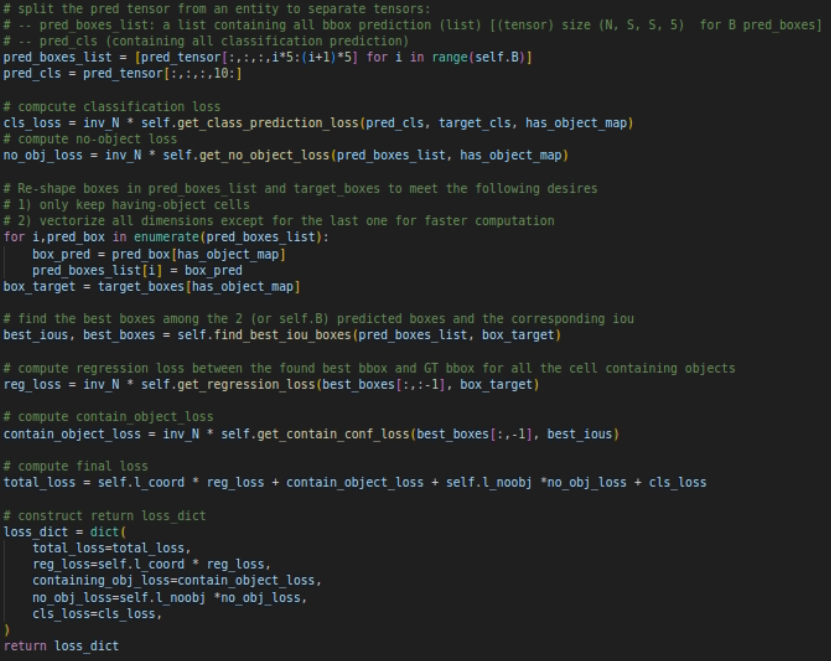
\includegraphics{code.png}}
    \caption{YOLO loss forward function}
    \label{fig:code}
  %\end{center}
  \vspace{0.1\baselineskip}
\end{figure}


\iffalse
\begin{table}[htb]
	\centering	
	\normalsize
    \newcommand{\z}{\phantom{0}}
    \caption{configurations of my experiment}
    \vspace{0.15\baselineskip}
    \resizebox{0.6\textwidth}{!}{
		\begin{tabular}[c]{|l|l|}
			\hline
			\textbf{parameter} & \textbf{configuration} \\
			\hline
			num\_epochs   &  45 \\
			\hline
			decay\_epochs & 15 \\
			\hline
			init\_lr & 0.01  \\
			\hline
			AdamW & weight\_decay = 0.01 \\
    			\hline
		\end{tabular}
	}
	\label{table:param}
   \vspace{0.1\baselineskip}
\end{table}
\fi


\section{準確度報告以及嘗試一些實驗}

\begin{table}[htb]
	\centering	
	\normalsize
    \newcommand{\z}{\phantom{0}}
    \caption{實驗測試}
    \vspace{0.15\baselineskip}
    %\resizebox{0.5\textwidth}{!}{
	\begin{tabularx}{0.6\textwidth}{@{}lr@{}}\toprule
		\textbf{Model} & \textbf{mAP} \\
		\hline
		resnet50 & \textbf{0.4691}  \\ 
		resnet50 + 水平翻轉 / 隨機擦除  & 0.2156  \\
    		\hline

	\end{tabularx}
	%}
	\label{table:comparison1}
   \vspace{0.15\baselineskip}
\end{table}


	我在epoch 45 的時候, validation set 上的測試結果達到最高的 mAP 是 0.4691。經過觀察,我發現大物體的AP較高,而小物體的較低,因此我嘗試了結合 focal loss,但效果沒有比較好,也嘗試了拿到訓練集我對影像做了RandomHorizontalFlip以及RandomErasing,想透過遮住一些物體來讓模型能夠更聚焦在其他物體或是其他輪廓上,但結果也沒有比較好。Table\ \ref{table:comparison1}呈現了我此次實驗的結果。

\iffalse
\begin{figure}[htb]
  \vspace{0.1\baselineskip}  
  \centering  
  %\begin{center}
    \resizebox{0.7\textwidth}{!}{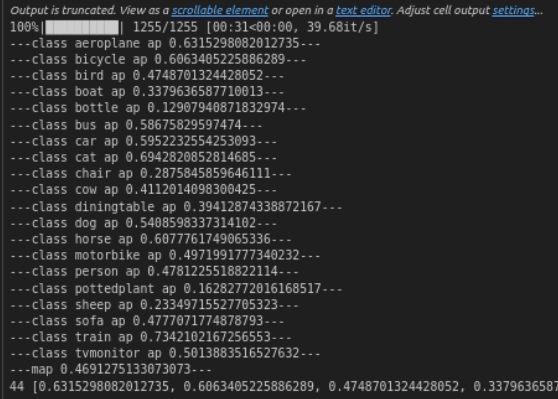
\includegraphics{output.png}}
    \caption{Best validation mAP on PASCAL}
    \label{fig:output}
  %\end{center}
  \vspace{0.1\baselineskip}
\end{figure}
\fi




\section{Extra credit}

\subsection{Video}
	這部分我主要實作方式是將影片的每一幀當做一個圖片來看待,每一幀送進我的模型偵測完後,經由 cv2 的套件將偵測結果畫上去,跟原來的幀做結合,在將每一幀輸出成影片,我的輸出影片連結有放在我的 A5.ipynb 裡面


\subsection{Train more advanced model \& other tricks} 
	由於剛剛在section 2 有討論過說,大物體小物體的feature scale不同,導致模型較關注大物體,因此針對這點,我想將 feature pyramid newtwork (FPN) 融入我的CNN架構中,來提取不同level的feature map,我的做法主要是分別對 ResNet50 裡面的四層的輸出結果提取出來,上層的layer的output經過上采樣後與下層的相加,在經過cnn結合起來,最後把得到的四個feature map經由插值resize到同一個大小在輸入detnet裡進行物件偵測,詳細程式碼在Figure\ \ref{fig:code2},但效果一樣不佳。

\begin{figure}[htb]
  \vspace{0.1\baselineskip}  
  \centering  
  %\begin{center}
    \resizebox{0.7\textwidth}{!}{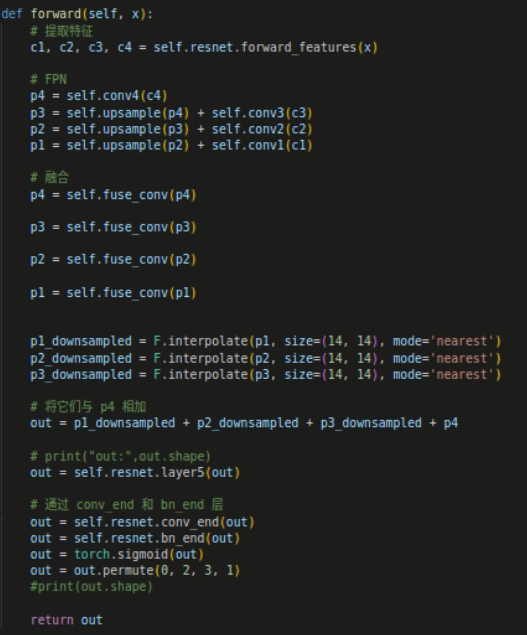
\includegraphics{code2.png}}
    \caption{implementation of FPN}
    \label{fig:code2}
  %\end{center}
  \vspace{0.1\baselineskip}
\end{figure}



\end{document}